\chapter{Probability}
\todo{take data from mathematical-tools course and put here.}

\section{Tricks and Techniques}

\paragraph{$\Pr{[A\cap B]}\ge ?$.}
Computing the exact probability of $A\cap B$ can be difficult, but we can often find a lower bound
by relying on the pidgenhole principle.

To compute it thus, we can write down the whole space, and plot it as a 
horizontal line starting at $0$ and ending at $1$.
then we plot a line to represent $A$. Given $A$ which starts from $0$ and ends at $a$,
we define $B$'s line as starting $1$ and ending at $b$ (see \autoref{probabilty:tricks:intersection}).

\begin{figure}
    % \centering
    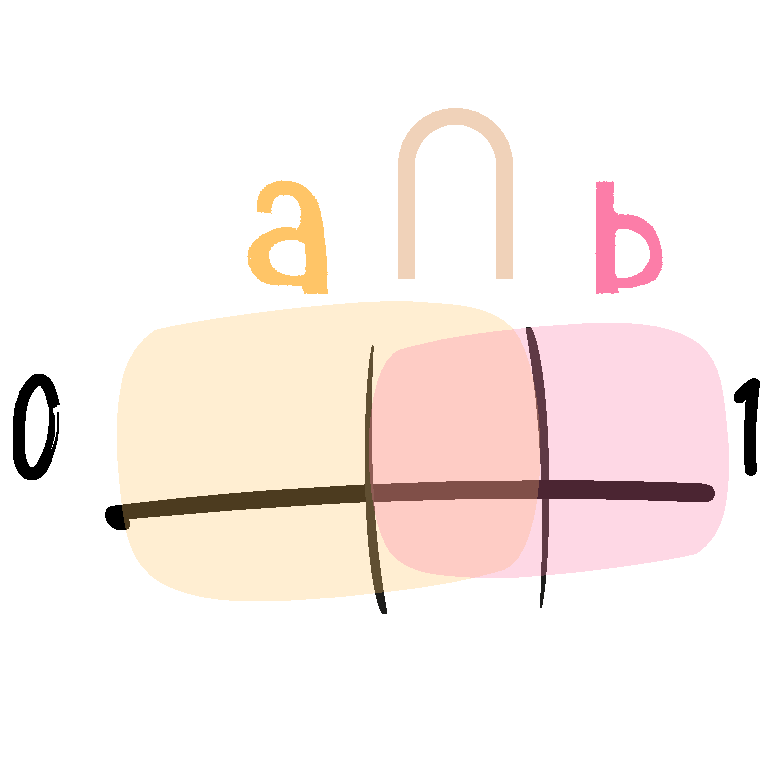
\includegraphics[scale=0.75]{mathematics/illustrations/AcapB.pdf}
\end{figure}\label{probabilty:tricks:intersection}

For example, $\Pr[A]=1-\frac{1}{16}, \Pr[B]=\frac{3}{4}$, thus, $A\cap B \ge \frac{3}{4}-\frac{1}{16}$. That is, 
We take the size of $B$ and remove $1-\Pr[A]$ from it.
